\chapter{Validation}

\section{Problem Description }

We aim to design and implement a new e-commerce system in this scenario. Based on business studies, the expected number of clients and their behavior are defined. The goal is to evaluate different architectural designs against non-functional requirements, particularly focusing on performance. The architecture team is exploring how many replications of the architecture they need to know how many replications need to satisfy the performance requirements.

\begin{figure}[H]
    \centering
    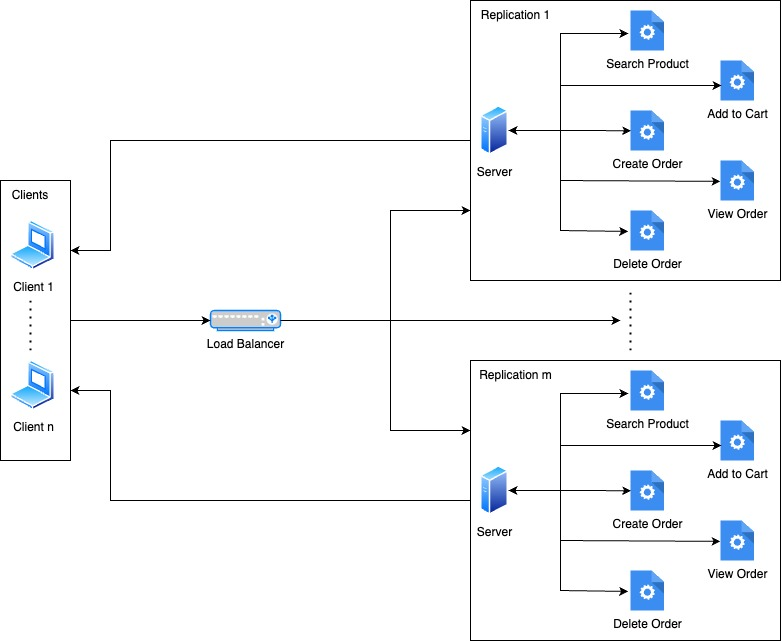
\includegraphics[width=1\linewidth]{images/archEcom.jpg}
    \caption{Eccomerce Software Design}
    \label{fig:eds}
\end{figure}

Line you can see, the architecture \ref{fig:eds} is divided in $m$ replication, and there is also a load balance \cite{loadBalancer} that will just randomacaly make connect a client to the server of a replication, than the client can make some requests based on their behaviour implemented with a markov chain \cite{markovChain}, also the load balancer can be considered as a DNS load Balancer.
\\ \\
And to define the behavior of the customer we can use a markov chain \ref{fig:markovchain}

\begin{figure}[H]
    \centering
    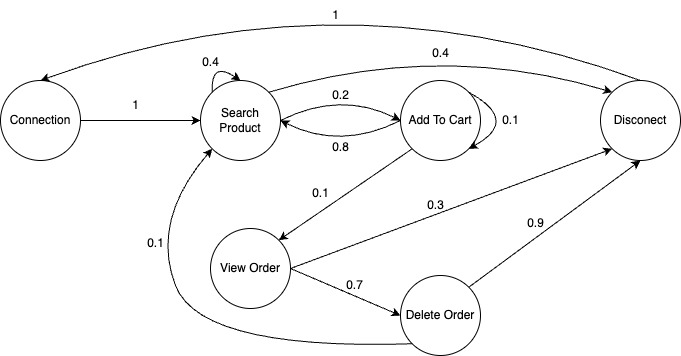
\includegraphics[width=\textwidth]{images/markovchain.jpg}
    \caption{Customer behaviour though Markov chain}
    \label{fig:markovchain}
\end{figure}


Now let's define the variables that will allow us to do the simulation and define the $SpeedUpSimulation$:
\begin{itemize}
    \item \( P = \begin{bmatrix}
                0 & 1 & 0 & 0 & 0 & 0 \\ 
                0 & 0.4 & 0.2 & 0 & 0 & 0.4 \\ 
                0 & 0.8 & 0.1 & 0.1 & 0 & 0 \\ 
                0 & 0 & 0 & 0 & 0.7 & 0.3 \\
                0 & 0.1 & 0 & 0 & 0 & 0.9 \\ 
                1 & 0 & 0 & 0 & 0 & 0
            \end{bmatrix} \)
    
    %\item \( svp = \begin{bmatrix} 0.20019036 & 0.47588832 & 0.10575296 & 0.0105753 & 0.00740271 & 0.20019036 \end{bmatrix} \)
    
    \item \( cst = \begin{bmatrix} 5 \times 86400 & 20 \times 60 & 16 \times 60 & 20 \times 60 & 1 \times 60 & 3600 \end{bmatrix}^{T} \)
    
    \item \( ast = \begin{bmatrix} 1 & 3 & 3 & 3 & 3 & 0 \end{bmatrix}^{T} \) 
    
    \item \( art = \begin{bmatrix} 0.3 & 0.7 & 0.4 & 0.5 & 0.4 & 0.1 \end{bmatrix}^{T} \)
    
    \item \( cmot = \begin{bmatrix} 10^{-7} & 10^{-7} & 10^{-7} & 10^{-7} & 10^{-7} & 10^{-7} \end{bmatrix}^{T} \)
    
    \item \( amot = \begin{bmatrix} 2 \times 10^{-7} & 2 \times 10^{-7} & 2 \times 10^{-7} & 2 \times 10^{-7} & 2 \times 10^{-7} & 2 \times 10^{-7} \end{bmatrix}^{T} \)
    
    \item \( network\_cost = 0.00023 \)
    
    \item \( cstoo = \begin{bmatrix} 4 & 3 & 3 & 3 & 3 & 1 \end{bmatrix}^{T} \)
    
    \item \( artoo = \begin{bmatrix} 3 & 9 & 9 & 9 & 9 & 2 \end{bmatrix}^{T} \)
    
    \item \( \theta = 5 \times 10^{-7} \)
    
    \item \( \beta = 1 \times 10^{-7} \)
    
    \item \( \alpha = 30 \)
\end{itemize}



\section{Non-functional Requirements}

Non-functional requirements (NFRs) define the quality attributes of a system, and they are critical for evaluating its performance, reliability, and maintainability. 
To 

Here, we will outline the key NFRs for our system, focusing on how they can be measured and how our simulation tool helps ensure performance qualities.

\begin{table}[H]
    \centering
    \small
    \renewcommand{\arraystretch}{1.5}
    \begin{tabular}{|c|c|c|c|c|}
        \hline
        \textbf{Server ID} & \textbf{Request Type} & \textbf{Request Time} & \textbf{Read Request} & \textbf{Response Time} \\
        \hline
        2100 & connection & 322.896095 & 322.896325 & 322.896555 \\
        \hline
        2100 & connection & 734.715306 & 734.715536 & 734.715766 \\
        \hline
        2100 & searchProduct & 966.871627 & 966.871857 & 967.572547 \\
        \hline
        2100 & searchProduct & 1066.145295 & 1066.145525 & 1066.846215 \\
        \hline
        2100 & searchProduct & 1432.340573 & 1432.340803 & 1433.041493 \\
        \hline
    \end{tabular}
    \caption{Request times and responses.}
    \label{tab:request_times}
\end{table}


Using the log structure (Table~\ref{tab:request_times}), we can calculate important metrics like minimum, maximum, mean, and variance for each request type, allowing us to assess the overall performance. These metrics give us insights into various NFRs, as explained below.

\subsection{Performance Metrics}

Performance is often the most critical non-functional requirement in systems handling large amounts of requests, as in our e-commerce scenario. We can calculate several performance-related metrics such as:

\begin{itemize}
    \item \textbf{Latency}: Time taken to process a request, measured from the logs.
    \item \textbf{Min, Max, Mean, and Variance}: Statistical measures to track response times, helping to identify performance bottlenecks.
\end{itemize}

\begin{table}[h!]
    \centering
    \renewcommand{\arraystretch}{1.5}
    \resizebox{!}{0.11\textwidth}{ % Adjust the height value (0.5\textheight) to compress vertically
        \begin{tabular}{|c|c|c|c|c|c|c|}
            \hline
            \textbf{Request Type} & \textbf{Min Request} & \textbf{Max Request} & \textbf{Mean Request} & \textbf{Var Request} & \textbf{Count Requests} \\
            \hline
            addToCart & 0.40092 & 0.630819 & 0.400996 & 1.745494e-05 & 3028 \\
            \hline
            connection & 0.00046 & 0.000460 & 0.000460 & 1.970162e-21 & 6539 \\
            \hline
            createOrder & 0.50092 & 0.500920 & 0.500920 & 2.117974e-21 & 300 \\
            \hline
            searchProduct & 0.70092 & 1.482193 & 0.702789 & 8.150574e-04 & 14197 \\
            \hline
            viewOrder & 0.40092 & 0.400920 & 0.400920 & 4.094827e-21 & 207 \\
            \hline
        \end{tabular}
    }
    \caption{Non-functional requirements results: Performance Analysis}
    \label{tab:request_statistics}
\end{table}


\subsection{Results and Observations}

We conducted tests with a range of values for \( p \) (number of client requests) and different values for \( c \) (number of clients), observing the simulation speed-up, \( SimulationSpeedup \). The goal is to determine when it is more convenient to use simulated-time simulations and when real-time simulations might be more efficient.

\begin{figure}[H]
    \centering
    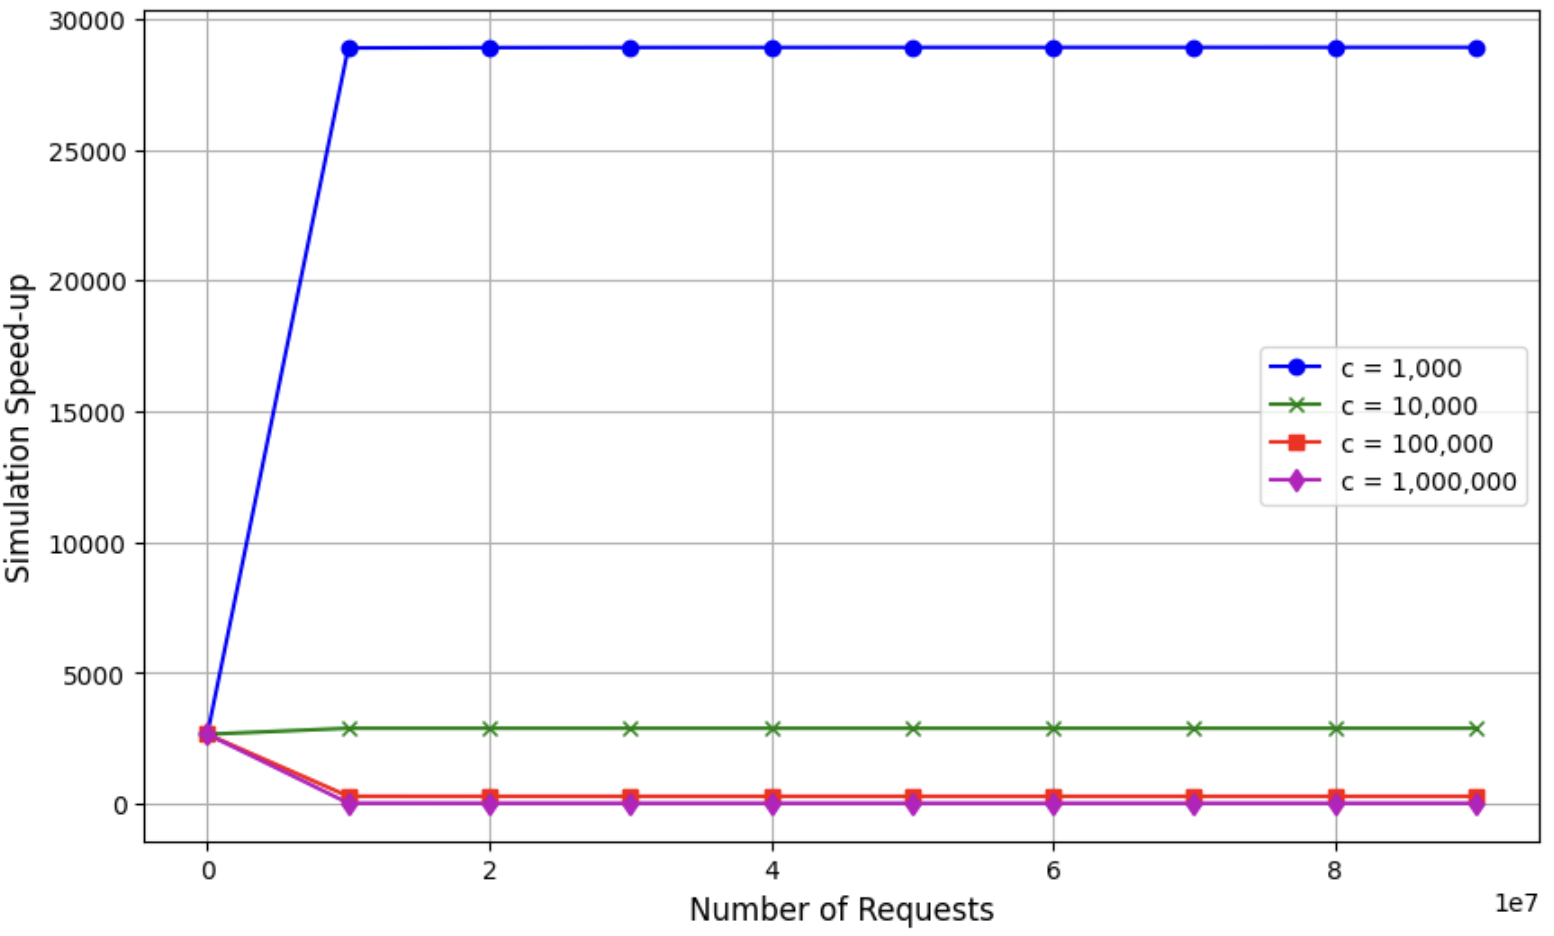
\includegraphics[width=\textwidth]{images/speed-up_result.png}
    \caption{Performance ratio}
    \label{fig:performance_ratio}
\end{figure}

Considering different values of \( c \) (number of clients), we observe that the simulation speed-up is significantly higher when the number of clients (\( c \)), is lower. This behavior is due to the parallel processing advantage of real-time simulations being less pronounced when there are fewer processes. With a lower number of clients, the overhead of coordinating real-time operations diminishes, making simulated time more efficient.

As the number of clients, \( c \), increases, real-time simulations become more efficient, and the total simulated time, \( T_{simulated} \), remains relatively unchanged. This is because real-time simulations can better distribute the workload across multiple machines.

Now lets' do see better if it's better than having a 10 times faster then real time\ref{fig:perfZoom}

\begin{figure}[H]
    \centering
    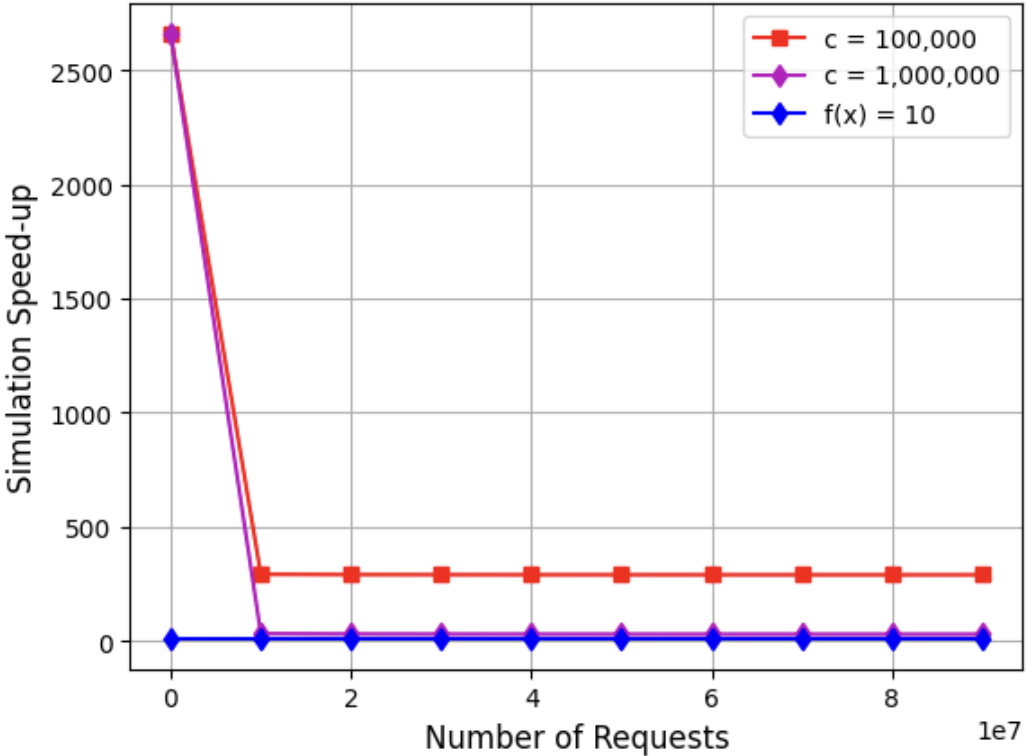
\includegraphics[width=\textwidth]{images/zoomgraph.png}
    \caption{Zoom on function with lower $SimulationSpeedUp$}
    \label{fig:perfZoom}
\end{figure}


We also sought to determine the maximum number of clients \( c \) that can handle at least 100,000,000 requests (\( p \)) while achieving a \( SimulationSpeedup \geq 10 \). Our findings indicate that \( c = 2,941,176 \) is required to achieve a speed-up of 10x in this scenario.

